%
%  D0018E report 1
%
%  Created by Anders Lindmark on 2012-10-31.
%  Copyright (c) 2011 Anders Lindmark. All rights reserved.
%
%\documentclass[]{article}
\documentclass[12pt, a4paper,titlepage]{article}

% Use utf-8 encoding for foreign characters
\usepackage[utf8]{inputenc}
\usepackage[english]{babel}

% Setup for fullpage use
\usepackage{fullpage}

\usepackage{float}

% Uncomment some of the following if you use the features
%
% Running Headers and footers
%\usepackage{fancyhdr}

% Multipart figures
%\usepackage{subfigure}

% More symbols
\usepackage{amsmath}
%\usepackage{amssymb}
%\usepackage{latexsym}

% Surround parts of graphics with box
\usepackage{boxedminipage}

% Package for including code in the document
\usepackage{listings}

% If you want to generate a toc for each chapter (use with book)
\usepackage{minitoc}

% This is now the recommended way for checking for PDFLaTeX:
\usepackage{ifpdf}

%\newif\ifpdf
%\ifx\pdfoutput\undefined
%\pdffalse % we are not running PDFLaTeX
%\else
%\pdfoutput=1 % we are running PDFLaTeX
%\pdftrue
%\fi

\ifpdf
\usepackage[pdftex]{graphicx}
\else
\usepackage{graphicx}
\fi

\usepackage{tikz}
\usetikzlibrary{positioning,arrows,fit,shapes,calendar,chains}
\usetikzlibrary{shadows}



\usepackage{tikz-er2} % For Entity-Relationship diagrams

\usepackage{pgfplots}
\usepackage{pgfplotstable}

\usepackage{hyperref}

\usepackage{enumerate}

\usepackage{todonotes}

%\usepackage{eso-pic}

\usepackage{color}
\definecolor{error}{RGB}{193,27,23} % #C11B17, Firebrick3
\definecolor{warning}{RGB}{229,103,23} % #E56717, Dark Orange2
\definecolor{codebg}{RGB}{245,245,245}
\definecolor{dkgreen}{rgb}{0,0.6,0}
\definecolor{poop}{rgb}{0.82,0.71,0.15}

\usepackage{parskip}
\setlength{\parskip}{0.4cm}
\setlength{\parindent}{0.6cm}

%\title{\huge\sffamily D7001D  Home examination}
%\author{Anders Lindmark, \emph{830604-8995}}
%\date{\today}

% http://tex.stackexchange.com/questions/16501/problem-with-special-characters-in-listings
%\lstset{literate=%
%{å}{{\aa}}1
%ä}{{\"a}}1
%{ö}{{\"o}}1
%{Å}{{\AA}}1
%{Ä}{{\"A}}1
%{Ö}{{\"O}}1
%}
\lstdefinelanguage{pseudo}{morekeywords={for,if,else,do,then,to,return,while,break}}
\lstset{
%backgroundcolor=\color{lightgray},
backgroundcolor=\color{codebg},
%title=\lstname,
frame=lines,
%inputencoding=utf8,
inputencoding=ansinew,
extendedchars=\true,
%basicstyle=\small,
basicstyle=\small,
commentstyle=\color{red},
numberstyle=\footnotesize,
stringstyle=\color{poop},
breaklines=true,
%keywordstyle=\color{black}\bfseries,
language=Python,
numbers=left,
}


\begin{document}
\ifpdf
\DeclareGraphicsExtensions{.pdf, .jpg, .tif}
\else
\DeclareGraphicsExtensions{.eps, .jpg}
\fi

\begin{titlepage}
\ 
\begin{center}
\vfill
{\huge\sffamily D0018E Report (2)}
\rule{\linewidth}{0.3mm}\\
Anders Lindmark \\
\vfill
\ 
\vfill
{\textbf{\today}}
\end{center}
\end{titlepage}

\tableofcontents
\newpage

\section{Establish a minimalistic website}
\subsection{Development environment}
The framework I have chosen to use is
Django\footnote{\url{https://www.djangoproject.com/}}. 
It is a framework that I have previous experience with and which I think is
very powerful aswell as easy to get started with.
It has a very good object-relational mapper (ORM) for working with databases as well
as support for running raw SQL-queries which are then mapped into objects
automatically using the ORM.

There are probably many good IDE's for developing in python/Django, NetBeans
being the one I usually use, but I will work with the editor \emph{vim}. It is the 
editor I'm most comfortable with, and vim combined with
\emph{screen}\footnote{\url{http://www.gnu.org/software/screen/}} and an
ssh-client enables me to switch computers and continue working where I left
off without having to install an IDE and download/upload code.

I will use \emph{git}\footnote{\url{http://git-scm.com/}} to keep track of code
and documentation changes which also enables me to go back to a point in
time incase I forget to document something in one of these hand-ins.

\subsection{The database}
Since I am developing on my own server I will use the 
\emph{MySQL}-installation already present on it.
I have started modelling the tables that I think I need for this application, using
the Django modelling system. When using this system you define a set of 
objects that represent the different tables and their columns. You can easily
specify relationships between the tables aswell. 

\subsubsection{Django models}
\label{sec:djangomodels}
The models that I have come up with so far, and these might change in the
future when more work is done, are:

\begin{itemize}
\setlength\itemsep{-1pt}
\item Customer - A user on the site. Django has a user-system already and this
model extends that system with the extra information we need.
\begin{lstlisting}
class Customer(models.Model):
    """ 
    Contains extra information about a customer other than the fields that are available in django-auth.
    """
    # For now, store all address info in one field, i.e "Bob Bobster\n13Bob street\nBobtown"
    address = models.CharField(max_length=150) 
    phone_number = models.CharField(max_length=20)
    user = models.OneToOneField(User) # The user-field points into Django's own auth-system.
\end{lstlisting}

\item Category - Different categories of products
\begin{lstlisting}
class Category(models.Model):
    """ 
    Represents a group of specific assets, i.e if we are selling food then "Snacks" could be a category
    """
    name = models.CharField(max_length=50)
    description = models.CharField(max_length=150)
\end{lstlisting}

\item Asset - The different products themselves
\begin{lstlisting}
class Asset(models.Model):
    """ 
    Represents a product.
    """
    name = models.CharField(max_length=50)
    description = models.CharField(max_length=150)
    category = models.ForeignKey(Category) # Which category does this asset belong to
    stock = models.IntegerField() # How many of this asset are in stock
\end{lstlisting}

\item Basket - The current shopping basket for a specific customer
\begin{lstlisting}
class Basket(models.Model):
    """
    Shopping basket, contains a list of assets and which customer it belongs to.
    """
    assets = models.ManyToManyField(Asset)
    customer = models.ForeignKey(Customer)
\end{lstlisting}

\item Order - A placed order
\begin{lstlisting}
class Order(models.Model):
    """
    A placed order, contains information about which assets was ordered, which customer placed the order and
    when the order was placed/shipped.
    """
    assets = models.ManyToManyField(Asset)
    customer = models.ForeignKey(Customer)
    date_placed = models.DateTimeField(auto_now=True) # Date the order was placed
    date_filled = models.DateTimeField() # Date the order was filled 
\end{lstlisting}
\end{itemize}

\subsubsection{SQL models}
\label{sec:sqlmodels}
Django takes the models that you have created and outputs SQL-code.
Normally this is done behind the scenes but you can get the SQL-code used
to create the tables. The code for the current version of my models looks like
this:

\lstset{language=SQL}
\begin{lstlisting}
CREATE TABLE `shopping_customer` (
    `id` integer AUTO_INCREMENT NOT NULL PRIMARY KEY,
    `address` varchar(150) NOT NULL,
    `phone_number` varchar(20) NOT NULL,
    `user_id` integer NOT NULL UNIQUE
)
;
ALTER TABLE `shopping_customer` ADD CONSTRAINT `user_id_refs_id_40cf930a` FOREIGN KEY (`user_id`) REFERENCES `auth_user` (`id`);

CREATE TABLE `shopping_category` (
    `id` integer AUTO_INCREMENT NOT NULL PRIMARY KEY,
    `name` varchar(50) NOT NULL,
    `description` varchar(150) NOT NULL
)
;
CREATE TABLE `shopping_asset` (
    `id` integer AUTO_INCREMENT NOT NULL PRIMARY KEY,
    `name` varchar(50) NOT NULL,
    `description` varchar(150) NOT NULL,
    `category_id` integer NOT NULL,
    `stock` integer NOT NULL
)
;
ALTER TABLE `shopping_asset` ADD CONSTRAINT `category_id_refs_id_71ff6d8a` FOREIGN KEY (`category_id`) REFERENCES `shopping_category` (`id`);

CREATE TABLE `shopping_basket_assets` (
    `id` integer AUTO_INCREMENT NOT NULL PRIMARY KEY,
    `basket_id` integer NOT NULL,
    `asset_id` integer NOT NULL,
    UNIQUE (`basket_id`, `asset_id`)
);
ALTER TABLE `shopping_basket_assets` ADD CONSTRAINT `asset_id_refs_id_4c78df9` FOREIGN KEY (`asset_id`) REFERENCES `shopping_asset` (`id`);

CREATE TABLE `shopping_basket` (
    `id` integer AUTO_INCREMENT NOT NULL PRIMARY KEY,
    `customer_id` integer NOT NULL
);
ALTER TABLE `shopping_basket` ADD CONSTRAINT `customer_id_refs_id_20577cdd` FOREIGN KEY (`customer_id`) REFERENCES `shopping_customer` (`id`);
ALTER TABLE `shopping_basket_assets` ADD CONSTRAINT `basket_id_refs_id_1faa067c` FOREIGN KEY (`basket_id`) REFERENCES `shopping_basket` (`id`);

CREATE TABLE `shopping_order_assets` (
    `id` integer AUTO_INCREMENT NOT NULL PRIMARY KEY,
    `order_id` integer NOT NULL,
    `asset_id` integer NOT NULL,
    UNIQUE (`order_id`, `asset_id`)
);
ALTER TABLE `shopping_order_assets` ADD CONSTRAINT `asset_id_refs_id_4d2211a4` FOREIGN KEY (`asset_id`) REFERENCES `shopping_asset` (`id`);

CREATE TABLE `shopping_order` (
    `id` integer AUTO_INCREMENT NOT NULL PRIMARY KEY,
    `customer_id` integer NOT NULL,
    `date_placed` datetime NOT NULL,
    `date_filled` datetime NOT NULL
);
ALTER TABLE `shopping_order` ADD CONSTRAINT `customer_id_refs_id_28221386` FOREIGN KEY (`customer_id`) REFERENCES `shopping_customer` (`id`);
ALTER TABLE `shopping_order_assets` ADD CONSTRAINT `order_id_refs_id_29c844c0` FOREIGN KEY (`order_id`) REFERENCES `shopping_order` (`id`);
\end{lstlisting} 
Here you can also see how it adds relationships between the tables.

\subsection{The website}
I would like to prefix this part by stating that I am not a good designer,
so the webpage that you see might make your eyes hurt a bit.

\subsubsection{Tools}
At its current state, the website uses HTML, CSS and JavaScript. 
I am using JQuery\footnote{\url{http://jquery.com/}} as the JavaScript-library
because I have previous experience with it and it makes things alot easier and
more convenient when developing and has good tools for using AJAX.

\subsubsection{The result}

I have created a very basic skeleton of a website that I think has all the pieces
I need for this application. I started by thinking about what components are
needed. I came up with this list:
\begin{description}
\setlength\itemsep{-5pt}
\item[Header] A place to put the logo of the webshop
\item[Footer] A place to end the webpage and put short, basic, information
		about it
\item[Navigation] A place to put global links, such as ``My Account'' and ``Shopping basket''.
\item[Body] The body needs two components, two columns, where the first
	column is a category-list and the second column is the main content page.
	The main content page contains information about the current product
	or the shopping basket, etc.
\end{description}

I also wanted you to be able to see the contents of the shopping basket at a
glance, my current solution for this is hovering the mouse over the shopping
basket link which toggles the visibility of a \emph{\lstinline{<div>}}-container.
In the future this will be done using an ajax call to a webpage that displays
information about the customers current shopping basket.

The website in it's current state can be seen here: \url{http://localghost.net/d0018e/1/}. 
A small screenshot can be seen in figure \ref{fig:sshot}.
\begin{figure}
\centering
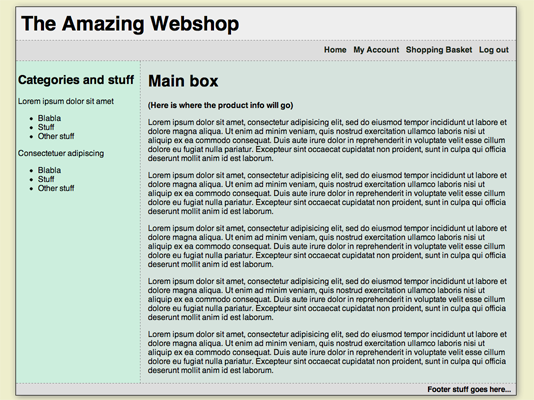
\includegraphics[width=10cm]{Screenshot_2012-11-16.png}
\caption{Screenshot of the webpage on November 16, 2012}
\label{fig:sshot}
\end{figure}

\subsubsection{References}
I used this guide:
\url{http://www.456bereastreet.com/lab/developing_with_web_standards/csslayout/2-col/}
when creating the website, it shows how to do a simple two-column webpage.

I used the CSS-information on \url{http://www.w3schools.com/} as a reference.

JQuery has excellent documentation available on \url{http://docs.jquery.com/}
and for positioning the shopping-basket information I used this addon: 
\url{http://docs.jquery.com/UI/API/1.8/Position}

\subsubsection{Converting the page to Django-templates}
The static skeleton-page has been converted into Django-templates.\todo[inline]{TODO: Include code and examples of the templates and show how inheritance, content-blocks etc works in Django}


\subsection{Content management system}
The basic point of a CMS is to separate the administration of the website and
the editing of webpage code from the content. This allows users to edit the
webpage while focusing on the content and not the other details surrounding
a large site, especially the details of editing html and styling the content.


\section{Establish a relational database for e-commerce}
\subsection{Schema}
Since I have created the models in the last handin 
(sections \ref{sec:djangomodels} and \ref{sec:sqlmodels})
I will now create an ER-diagram based on those specifications.

My schema consists of these entities:
\begin{itemize}
\setlength\itemsep{-5pt}
\item Customer
\item Category
\item Asset
\item Basket
\item Order
\end{itemize}
There is one additional entity which has a relationship to my model but isn't
defined by me. This is the \emph{User} entity that belongs to Django that I
extend using the Customer entity.

The relationships between these entities are as follows:
\begin{itemize}
\setlength\itemsep{-5pt}
\item \emph{Customer} extends \emph{User}
\item \emph{Asset} belongs to a \emph{Category}
\item \emph{Basket} contains \emph{Asset}s
\item \emph{Basket} belongs to a \emph{Customer}
\item \emph{Order} contains \emph{Asset}s
\item \emph{Order} belongs to a \emph{Customer}
\end{itemize}
\emph{Order} and \emph{Basket} have the same relationships. This is because
an order is essentially a saved \emph{Basket}. The schema could be simplified
by removing \emph{Order} altogether and adding an attribute to \emph{Basket}
which indicates whether the contents of the basket has been ordered or not.
I have chosen not to do this for now, because \emph{Order} also contains
information about when the order was placed/filled, and it seems a waste to
add these three fields (is\_order, date\_placed, date\_filled) to every
\emph{Basket} row. This might change in the future.


\subsubsection{Entity-Relationship Diagram}
The entity-relationship diagram created from this information and with the
attributes of the entities added can be seen in figure \ref{fig:erdiag}. 
The meaning of the different symbols is explained in this figure:
\begin{figure}[H]
\centering
\tikzstyle{every entity} = [top color=white, bottom color=blue!30, 
                            draw=blue!50!black!100, drop shadow]
\tikzstyle{every attribute} = [top color=white, bottom color=yellow!20, 
                               draw=yellow, node distance=1cm, drop shadow]
\tikzstyle{every relationship} = [top color=white, bottom color=green!20, 
                                  draw=green!50!black!100, drop shadow]
\begin{tikzpicture}[node distance=0.5cm, every edge/.style={link}]
% Legend
\node[entity] (leg_ent) [scale=0.65] {Entity};
\node[relationship] (leg_rel) [scale=0.65, right=of leg_ent] {Relationship};
\node[attribute] (leg_att) [scale=0.65, right=0.5cm of leg_rel] {Attribute};
%\node[draw,dashed,fit=(leg_ent) (leg_rel) (leg_att)] (leg_box) {};
\end{tikzpicture}
\caption{Legend for the ER-diagram (figure \ref{fig:erdiag})}
\end{figure}

\begin{figure}[H]
\centering
\tikzstyle{every entity} = [top color=white, bottom color=blue!30, 
                            draw=blue!50!black!100, drop shadow]
\tikzstyle{every attribute} = [top color=white, bottom color=yellow!20, 
                               draw=yellow, node distance=1cm, drop shadow]
\tikzstyle{every relationship} = [top color=white, bottom color=green!20, 
                                  draw=green!50!black!100, drop shadow]
\begin{tikzpicture}[node distance=1.5cm, every edge/.style={link}]
\node[entity] (cust) {Customer};
\node[relationship] (custusr) [above=of cust] {\,\,\,Extends\,\,\,\,} edge (cust);
\node[entity] (user) [bottom color=black!20, draw=black!40!black!60, dotted] [above=of custusr] {User} edge (custusr);

\node[entity] (asset) [right=5 cm of cust] {Asset};
\node[relationship] (asscat) [above=of asset] {Belongs to} edge (asset);
\node[entity] (category) [above=of asscat] {Category} edge (asscat);

\node[relationship] (ordcus) [below left=1.5 cm and 1 cm of cust] {Belongs to} edge (cust);
\node[relationship] (ordass) [below left=1cm and 0.2cm of asset] {\,\,\,Contains\,\,\,} edge (asset);

\node[relationship] (bascus) [below right=1cm and 0.2cm of cust] {Belongs to} edge (cust);
\node[relationship] (basass) [below right=1.5cm and 1cm of asset] {\,\,\,Contains\,\,\,} edge (asset);

\node[entity] (order) [below right=2cm and 3cm of ordcus] {Order} edge (ordcus) edge (ordass);
\node[entity] (basket) [below left=2cm and 3cm of basass] {Basket} edge (bascus) edge (basass);

% Customer attributes
\node[attribute] (address) [above left=1.25cm and 0.5cm of cust] {Address} edge (cust);
\node[attribute] (phone) [above left=0.25cm and 1.5cm of cust] {Phone} edge (cust);

% Asset attributes
\node[attribute] (name) [above right=1.25cm and 0.5cm of asset] {Name} edge (asset);
\node[attribute] (desc) [above right=0.25cm and 1.5cm of asset] {Description} edge (asset);
\node[attribute] (stock) [above right=-1cm and 1.5cm of asset] {Stock} edge (asset);

% Order attributes
\node[attribute] (dateordered) [below left=0.5cm and 1.5cm of order] {Order placed} edge (order);
\node[attribute] (datefilled) [below left=1.25cm and -2cm of order] {Order filled} edge (order);

% Category attributes
\node[attribute] (cname) [above left=1cm and 0cm of category] {Name} edge (category);
\node[attribute] (cdesc) [above right=1cm and 0cm of category] {Description} edge (category);
\end{tikzpicture}
\caption{Entity-relationship diagram}
\label{fig:erdiag}
\end{figure}


\subsection{Use cases}
I have tried to think of a few different use cases that might be typical for the
people interacting with the webshop. I'm not entirely sure that I structured
the use-cases correctly, or if the use-case diagram (figure \ref{fig:usecase}) is
correctly designed.

\subsubsection{Browse category}

\begin{table}[H]
\centering
\begin{tabular}{r | p{12cm}}
\textbf{Title} & Browse category \\
\textbf{Actor} & User \\
\textbf{Goal} & Retrieve a list of all the products associated with a certain category \\
\textbf{Story} & The user clicks on one of the categories available from the sidebar and a new page is opened with a list of products \\
\end{tabular}
\caption{Browse category use-case}
\end{table}

\subsubsection{Purchase item}
\begin{table}[H]
\centering
\begin{tabular}{r | p{12cm}}
\textbf{Title} & Purchase item \\
\textbf{Actor} & User \\
\textbf{Goal} & Add an item to the shopping basket \\
\textbf{Story} & The user clicks on the purchase link/icon assiciated with the selected product and the product is added to the shopping basket\\
\end{tabular}
\caption{Purchase item use-case}
\end{table}

\subsubsection{Place order}
\begin{table}[H]
\centering
\begin{tabular}{r | p{12cm}}
\textbf{Title} & Place order \\
\textbf{Actor} & User \\
\textbf{Goal} & Place an order containing all of the items in the shopping basket \\
\textbf{Story} & The user is satisfied with the products in the shopping basket and opens the basket page by clicking on the link in the navigation panel.
A page showing order-confirmation with address and payment details is opened \\
\end{tabular}
\caption{Place order use-case}
\end{table}

\subsubsection{Fill order}
\begin{table}[H]
\centering
\begin{tabular}{r | p{12cm}}
\textbf{Title} & Fill order \\
\textbf{Actor} & Warehouse worker \\
\textbf{Goal} & Fill an order that is waiting for processing \\
\textbf{Story} & The warehouse worker opens a webpage that contains a list of
unprocessed orders, selects the one that has been waiting for the longest time and is shown a page where all the items, item-counts and customer shipping
details are shown. 
After retrieving all the ordered items and posting the box  the warehouse worker marks the order as placed\\
\end{tabular}
\caption{Fill order use-case}
\end{table}

\subsubsection{Change address}
\begin{table}[H]
\centering
\begin{tabular}{r | p{12cm}}
\textbf{Title} & Change address \\
\textbf{Actor} & User \\
\textbf{Goal} & Edit the address information stored in the database \\
\textbf{Story} & The user has moved to a new address and wishes to update
the information stored in the webshop. The user clicking on \emph{My Account}
in the navigation panel, edits the text-field with the address information and
clicks save \\
\end{tabular}
\caption{Fill order use-case}
\end{table}

\subsubsection{Add product}
\begin{table}[H]
\centering
\begin{tabular}{r | p{12cm}}
\textbf{Title} & Add product \\
\textbf{Actor} & Manager \\
\textbf{Goal} & Add a new product to the webshop \\
\textbf{Story} & A contract with a new supplier has been signed and new products need to be added to he shop. The manager goes to the administrative page and selects add product. A webform is presented where the manager enters the product information and uploads a picture \\
\end{tabular}
\caption{Add product use-case}
\end{table}

\subsubsection{Use-case diagram}
\begin{figure}[H]
\centering
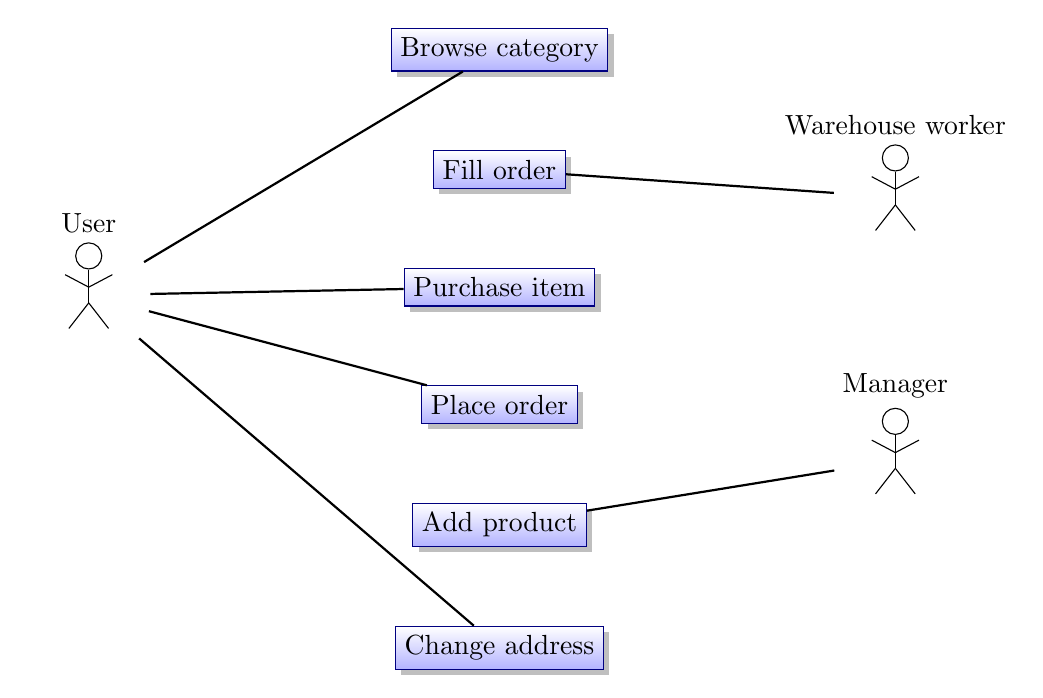
\begin{tikzpicture}[node distance=1cm]
% User
\node [draw, circle] (head1) {};
\node [below=0.3cm of head1] (midriff1) {};
\node [below=0.1cm of head1] (chestnode1) {};
\coordinate (mid1) at (midriff1);
\coordinate (chest1) at (chestnode1);
\node [below right=0.2cm and 0.1cm of midriff1] (rightleg1) {} edge (mid1);
\node [below left=0.2cm and 0.1cm of midriff1] (leftleg1) {} edge (mid1);
\draw  (mid1) -- (head1);
\node [above left=0.1cm and 0.3cm of chest1] (leftarm1) {} edge (chest1);
\node [above right=0.1cm and 0.3cm of chest1] (rightarm1) {} edge (chest1);
\node [above=0cm of head1] (label1) {User};
\node [ellipse, inner sep=0cm, fit=(head1) (midriff1) (chestnode1) (rightleg1) (leftleg1) (leftarm1) (rightarm1)] (personbox1) {};

% Use cases
%\node [draw] [right=4cm of chest1] [top color=white, bottom color=blue!30, draw=blue!50!black!100, drop shadow] 
%	(place) {Place order};
\node [draw] [right=4cm of chest1] [top color=white, bottom color=blue!30,  draw=blue!50!black!100, drop shadow] 
	(purchase) {Purchase item};
\node [draw] [above=of purchase] [top color=white, bottom color=blue!30,  draw=blue!50!black!100, drop shadow] 
	(fill) {Fill order};
\node [draw] [above=of fill] [top color=white, bottom color=blue!30,  draw=blue!50!black!100, drop shadow] 
	(browse) {Browse category};
%\node [draw] [below=of place] [top color=white, bottom color=blue!30,  draw=blue!50!black!100, drop shadow] 
%	(purchase) {Purchase item};
\node [draw] [below=of purchase] [top color=white, bottom color=blue!30, draw=blue!50!black!100, drop shadow] 
	(place) {Place order};
\node [draw] [below=of place] [top color=white, bottom color=blue!30,  draw=blue!50!black!100, drop shadow] 
	(addproduct) {Add product};
\node [draw] [below=of addproduct] [top color=white, bottom color=blue!30,  draw=blue!50!black!100, drop shadow] 
	(change) {Change address};

% User connections
\draw [thick] (personbox1) -- (browse);
\draw [thick] (personbox1) -- (purchase);
\draw [thick] (personbox1) -- (place);
\draw [thick] (personbox1) -- (change);

% Warehouse worker
\node [draw, circle] [above right=1cm and 10cm of head1]  (head2) {};
\node [below=0.3cm of head2] (midriff2) {};
\node [below=0.1cm of head2] (chestnode2) {};
\coordinate (mid2) at (midriff2);
\coordinate (chest2) at (chestnode2);
\node [below right=0.2cm and 0.1cm of midriff2] (rightleg2) {} edge (mid2);
\node [below left=0.2cm and 0.1cm of midriff2] (leftleg2) {} edge (mid2);
\draw  (mid2) -- (head2);
\node [above left=0.1cm and 0.3cm of chest2] (leftarm2) {} edge (chest2);
\node [above right=0.1cm and 0.3cm of chest2] (rightarm2) {} edge (chest2);
\node [above=0cm of head2] (label2) {Warehouse worker};
\node [ellipse, inner sep=0cm, fit=(head2) (midriff2) (chestnode2) (rightleg2) (leftleg2) (leftarm2) (rightarm2)] (personbox2) {};

% Warehouse worker connections
\draw [thick] (personbox2) -- (fill);

% Manager
\node [draw, circle] [below=3cm of head2]  (head3) {};
\node [below=0.3cm of head3] (midriff3) {};
\node [below=0.1cm of head3] (chestnode3) {};
\coordinate (mid3) at (midriff3);
\coordinate (chest3) at (chestnode3);
\node [below right=0.2cm and 0.1cm of midriff3] (rightleg3) {} edge (mid3);
\node [below left=0.2cm and 0.1cm of midriff3] (leftleg3) {} edge (mid3);
\draw  (mid3) -- (head3);
\node [above left=0.1cm and 0.3cm of chest3] (leftarm3) {} edge (chest3);
\node [above right=0.1cm and 0.3cm of chest3] (rightarm3) {} edge (chest3);
\node [above=0cm of head3] (label3) {Manager};
\node [ellipse, inner sep=0cm, fit=(head3) (midriff3) (chestnode3) (rightleg3) (leftleg3) (leftarm3) (rightarm3)] (personbox3) {};

% Manager connections
\draw [thick] (personbox3) -- (addproduct);
\end{tikzpicture}
\caption{Use-case diagram}
\label{fig:usecase}
\end{figure}

\subsection{Testing}
Some data is needed in the database to enable tests of the website.
Adding data to the database is currently done manually.

\subsubsection{Adding data to the database}
Django provides the ability to work with your application interactively through
the shell. This is very similar to working with an interactive python session but
also loads all the required Django-libraries.

To populate the database I have created this small script that is executed in the
django-shell environment:
\lstset{language=Python}
\begin{lstlisting}
from shopping.models import Customer, Category, Asset, Basket, Order

categories = [ 
        # (name, description)
        ('socks', 'Items to put on your feet'),
        ('shoes', 'Items to put on your socks'),
        ('fruit', "Eat this, it's good for you"),
        ('telephones', 'Put one end against your ear and shout in the other'),
]   

for n, d in categories:
    c = Category(name=n, description=d)
    c.save()

sockCat = Category.objects.get(name='socks')
shoeCat = Category.objects.get(name='shoes')
fruitCat = Category.objects.get(name='fruit')
telCat = Category.objects.get(name='telephones')
products = [ 
        # (name, description, category, stock)
        ('blue sock', 'An exquisite blue sock, fit for kings and queens alike', sockCat, 3), 
        ('green sock', 'A sock of the green persuasion', sockCat, 10),
        ('gray sock', 'This sock lacks color', sockCat, 7), 

        ('boot', 'A boot (or two boots to be specific)', shoeCat, 5), 
        ('loafer', 'A loafer, slip it on and forget all about it', shoeCat, 3), 
    
        ('banana', 'A yellow fruit, not very round at all', fruitCat, 24),
        ('pear', 'This fruit is a bit more round than the banana', fruitCat, 13),
        ('apple', "Currently this is the roundest fruit we've got!", fruitCat, 7), 

        ('fixed phone', "This is where it's at", telCat, 10),
        ('mobile phone', "Everywhere is where it's at", telCat, 10) 
]   

for n, d, c, s in products:
    a = Asset(name=n, description=d, category=c, stock=s)
    a.save()
\end{lstlisting}
This creates a number of categories and then a number of assets which
belong to the different categories.

\subsection{Goals for the upcoming sprint}
In the upcoming sprint I plan to:
\begin{itemize}
\setlength\itemsep{-5pt}
\item Extend the test-data to include customers, orders and shopping-baskets
\item Add more functionality to the website (i.e clicking ``buy'' on a product adds it to the shopping basket)
\item The product listings also needs to look better, and support images too. 
Whether the images should be stored as files or as an additional field in the
database is not yet decided.
\end{itemize}

\subsection{Tools and references}
The diagrams were created using the \LaTeX-package
``Ti\emph{k}Z'', which I've used before and is great in many ways for diagram
drawing and data plotting. The Ti\emph{k}Z-manual can be found here:
\url{http://www.texample.net/media/pgf/builds/pgfmanualCVS2012-11-04.pdf}
and there are plenty of different Ti\emph{k}Z-examples on this page:
\url{http://www.texample.net/tikz/examples/} (including an ER-diagram example).

\end{document}
